\documentclass[ngerman, a4paper,12pt]{article}

%\usepackage[applemac]{inputenc} % Bei Benutzung von Apple-Betriebssystemen bitte durch ``\usepackage[applemac]{inputenc}'' ersetzen.
\usepackage[utf8]{inputenc}
\usepackage[T1]{fontenc}
\usepackage{subcaption}
\usepackage[ngerman]{babel} 
\usepackage{fixltx2e}
\usepackage{tabularx}
\usepackage{booktabs}
\usepackage{placeins}
\usepackage{eurosym}
\usepackage{amssymb,amsmath}
\usepackage{mathtools}
\usepackage{graphicx} 
\usepackage{color}
\definecolor{kit}{cmyk}{1,0,0.6,0}

\usepackage{hyperref}
\hypersetup{pdftoolbar=true,
            pdfmenubar=true,
            pdfpagemode=UseOutlines,
            bookmarksnumbered=true,
            linktocpage=true,
            colorlinks=false,
            %backref, % Entkommentieren, um zu sehen, ob alle Literaturstellen im Text zitiert werden.
            colorlinks=false
            }

\newtheorem{definition}{Definition}[section]
\newtheorem{satz}[definition]{Satz}
\newtheorem{lemma}[definition]{Lemma}
\newtheorem{korollar}[definition]{Korollar}
\newtheorem{proposition}[definition]{Proposition}
\newtheorem{bemerkung}[definition]{Bemerkung}
\newtheorem{beispiel}[definition]{Beispiel}
\newtheorem{problem}[definition]{Problem}
\newtheorem{Voraussetzung}[definition]{Voraussetzung}
\newtheorem{algorithmus}[definition]{Algorithmus}
\newtheorem{vermutung}[definition]{Vermutung}

\setlength{\parindent}{0pt}
\parskip1.5ex

\newcommand{\R}{\mathbb R} % Beispiel für die Definition eines eigenen Befehls

\begin{document}

\begin{flushleft}
\vspace*{-100pt}
\textbf{Institut f\"ur Operations Research \\
Prof. Dr. Oliver Stein \\}
Sommersemester 2018
\vspace*{15pt}
\end{flushleft}

\begin{flushright}
\vspace*{-80pt}

\includegraphics[scale=0.5]{kit_logo}
\vspace*{15pt}
\end{flushright}

\begin{center}
\textbf{Zweite Bonusübung zur Vorlesung \\
\emph{Globale Optimierung I}}        
\end{center}

\begin{table}[h]
	\centering
	\begin{tabularx}{\textwidth}{X X X X X}
		 & Vorname & Nachname & Matr.Nr. & Bachelor / Master \\
		\toprule
		1. Mitglied & Leon & Qadirie & 1720201 &  Master\\
		2. Mitglied & Lukas & Kemmer & 1725171 &  Master\\
		\bottomrule
	\end{tabularx}
\end{table}
\textbf{Aufgabe S2.1} \\
(a) Das lineare Gleichungssystem
\begin{equation}
  (A^TA+\alpha R^TR)x=A^Tb
\end{equation}
besitzt genau dann eine eindeutige Lösung, wenn $A^TA+\alpha R^TR$ invertierbar ist. Weiterhin gilt
\begin{equation*}
	\begin{split}
		Kern(A^TA + \alpha R^T R) &= \{x \in \mathbb{R}^n \ | \ A^TAx + \alpha R^TRx = 0 \} \\
	&=\{x \in \mathbb{R}^n \ | \ x^TA^TAx + \alpha x^TR^TRx = 0 \} \\
	\end{split}
\end{equation*}
mit $x^TA^TAx = \| Ax \| _2^2 \geq 0$ und $\alpha x^TR^TRx = \alpha \| Rx \|_2^2 \geq 0$ (wegen $\alpha >0$). Damit folgt, dass 
\begin{equation}
	x^TA^TAx + \alpha x^TR^TRx = 0
\end{equation}
nur dann erfüllt ist, wenn beide Summanden $0$ sind, d.h. wir suchen ein $x$ für das sowohl $x^TA^TAx=0$ als auch $x^TR^TRx=0$ gilt (wegen $\alpha>0$ muss $\alpha$ hier nicht berücksichtigt werden). Aus
\begin{equation*}
	\begin{split}
		Kern(A) \cap Kern(B) &= \{x \in \mathbb{R}^n \ | \ Ax=0 \} \cap \{x \in \mathbb{R}^n \ | \ Rx=0 \} \\
		&=\{x \in \mathbb{R}^n \ | \ x^TA^TAx=0 \land x^TR^TRx=0 \} \\
		&=\{0\}
	\end{split}
\end{equation*}
folgt, dass diese Vorderung nur für $x=0$ erfüllt ist. Damit gilt $Kern(A^TA + \alpha R^TR) = \{0\}$ und damit nach Satz 5 der mathematischen Grundlagen, dass $A^TA + \alpha R^TR$ invertierbar ist (wir merken an, dass es sich um eine $(n \times n)$-Matrix handelt). Die eindeutige Lösung des linearen Gleichungssystems ist dann
\begin{equation*}
	\begin{split}
	(A^TA+\alpha R^TR)x &=A^Tb \\
	\Leftrightarrow x&= (A^TA+\alpha R^TR)^{-1} A^Tb	
	\end{split}
\end{equation*}
% und es folgt
%\begin{equation}
%	x = (A^TA+\alpha R^TR)^-1 A^Tb.
%\end{equation}
%Gemäß $A6$ besitzt $A^TA+\alpha R^TR$ vollen Rang, so $Kern(A^TA+\alpha R^TR=\{0\}$
%Kern(A)\cap Kern(R)=\{0\} \Rightarrow \{x\in \mathbb R^n|Ax=0\}\cap\{x\in\mathbb R^n|Rx=0\}
%Es gilt: $Kern(A^TA+\alpha R^TRx)$\\[10pt]
%=$\{x\in\mathbb R^n|(A^TA+\alpha R^TR)x=0\}$\\[10pt]
%=$\{x\in \mathbb R^n|\underbrace{A^TA}_{n\times n,\succeq 0}x\}+\alpha\underbrace{R^TR}_{n\times n,\succeq 0}x=0\}=\{0\}\quad$ \footnote{Positiv semidefinit da Gram-Matrix}\\[10pt]
%=$\{x\in \mathbb R^n|x^T\underbrace{A^TA}_{\geq 0}x\}+\alpha x^T\underbrace{R^TR}_{\geq 0}x=0\}=\{0\}$\\[10pt]
%da nur für $x=0:(Ax=0)\wedge (Rx=0)$.
%\textcolor{red}{Damit ist $A^TA+\alpha R^TR$ invertierbar}
\par
(b) Sei $f: \mathbb{R}^n \rightarrow \mathbb{R}$ mit $f(x) = \|Ax-b \|_2^2 + \alpha \|Rx \|_2^2$. Wegen $D^2( \|x \|_2^2)=2I \succeq 0$, der Linearität von $Ax-b$ sowie $Rx$ und $\alpha > 0$ folgt mit Übungen 4.4, 4.6 und Satz 2.5.3 die Konvexität von $f$ als Summe konvexer Funktionen (merke, dass es sich um ein unrestringiertes Problem mit $M=\mathbb{R}^n$ handelt und der $\mathbb{R}^n$ eine konvexe Menge ist). Mit Satz 2.4.5 und Korollar 2.4.6 folgt, dass die kritischen Punkte von $f$ genau die globalen Minimalpunkte sind. Es gilt
\begin{equation}
	\nabla f(x) = 2A^T(Ax-b) + 2\alpha R^TRx
\end{equation}
und damit
\begin{equation*}
	\begin{split}
		2A^T(A\bar{x}-b) + 2\alpha R^TR\bar{x} &= 0 \\
		\Leftrightarrow A^TA\bar{x}-A^Tb+\alpha R^TR\bar{x} &=0 \\
		\Leftrightarrow (A^TA+\alpha R^TR)\bar{x} &=A^Tb \\
		\Leftrightarrow \bar{x} &= (A^TA+\alpha R^TR)^{-1}A^Tb.
	\end{split}
\end{equation*}
Damit ist die eindeutige Lösung des linearen Gleichungssystems aus (a) genau der eindeutige globale Minimalpunkt von $P$.
%Es handelt sich bei dem Gleichungssystem aus (a) offensichtlich um ein konvexes Optimierungsproblem.
%Entsprechend sind alle kritischen Punkte auch Nullstellen.
%Es gilt:
%$\nabla_x f(x)=A^T(Ax-b)+\alpha R^TRx\stackrel{!}{=}0$\\[5pt]
%$\Leftrightarrow A^TAx-A^Tb+\alpha R^TRx=0$\\[5pt]
%$\Leftrightarrow (A^TA+\alpha R^TR)x=A^Tb$\\[5pt]
%q.e.d.
\par
\textbf{Aufgabe S2.2} \\
(a) Das lineare Gleichungssystem aus S2.1 (a) kann gelöst werden mit $R \coloneqq L, \ b \coloneqq y, \ A \coloneqq I$ wobei
%R:=L, \textcolor{red}{b:=Y}, A:=I.
\begin{equation*}
	L = \begin{pmatrix}
	1 &-1 & 0 \cdots &0 &0\\
	0 & 1 & -1 \cdots &0 &0\\
	\vdots & \vdots & \vdots & \vdots & \vdots \\
	0 & 0 & \cdots & 1 & -1\\ 
	\end{pmatrix} \in \mathbb R^{(n-1)\times n}.
\end{equation*}
Der Rest der Lösung ist in dem angehängten Python-Code dokumentiert.
\par
(b) Die Ergebnisse aus $RL_2$ sind in Abbildung $1$ dargestellt. 
\begin{figure}[h]
	\centering
	\label{fig:s22}
	\begin{subfigure}[b]{0.45\textwidth}
		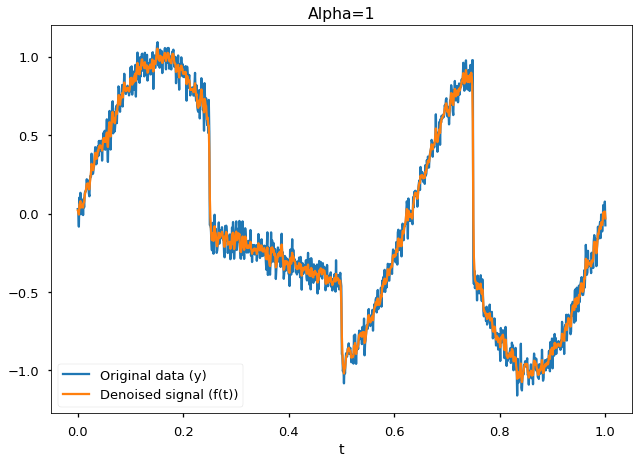
\includegraphics[width=1\columnwidth]{Images/2a1.png}
		\label{2a1}
	\end{subfigure}
	\begin{subfigure}[b]{0.45\textwidth}
		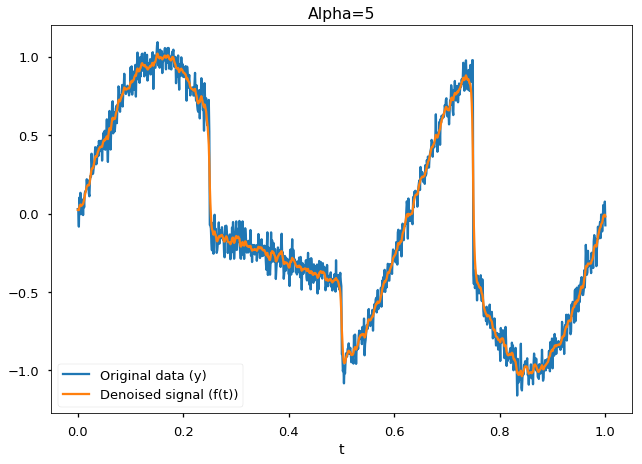
\includegraphics[width=1\columnwidth]{Images/2a5.png}
		\label{2a5}
	\end{subfigure}
	\begin{subfigure}[b]{0.45\textwidth}
		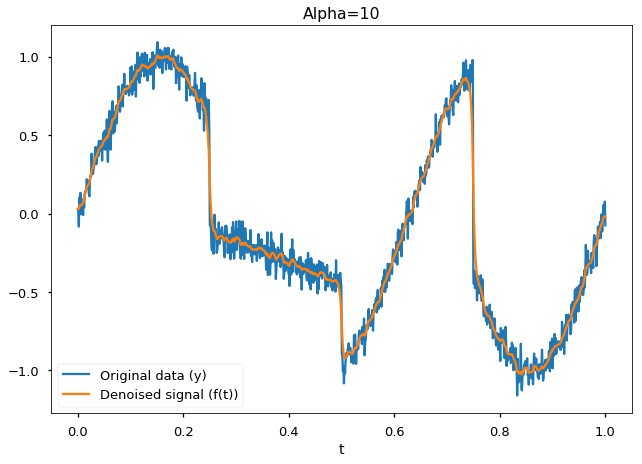
\includegraphics[width=1\columnwidth]{Images/2a10.png}
		\label{2a10}
	\end{subfigure}
	\begin{subfigure}[b]{0.45\textwidth}
		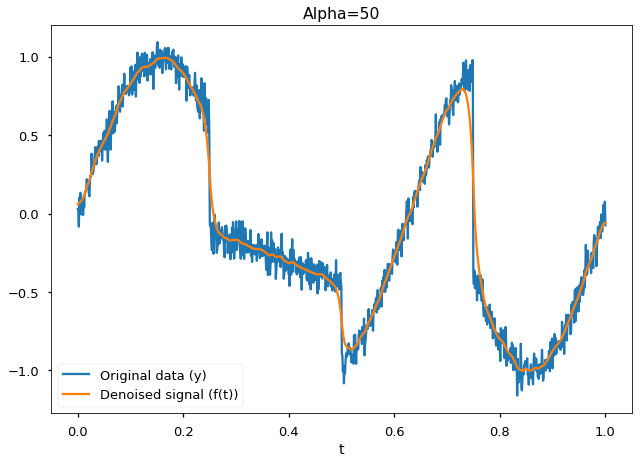
\includegraphics[width=1\columnwidth]{Images/2a50.png}
		\label{2a50}
	\end{subfigure}
	\caption{Ergebnisse aus $RL_2$ mit $\alpha \in \{1, 5, 10, 50\}$.}
	\vspace{-20pt}
\end{figure}
Mithilfe von $RL_2$ erhalten wir Approximationen der Werte $f(t_k)$ die augenscheinlich einer glatten Funktion ähneln. Bei Betrachtung der zugrunde liegenden Daten können jedoch drei potentielle Sprungstellen identifiziert werden, bei denen die Sprünge deutlich stärker ausfallen als das sonst vorliegende Rauschen. Es ist daher fraglich, ob es sich bei dem Ergebnis von $RL_2$ um eine gute Approximation handelt. Darüber hinaus sollte beachtet werden, dass das Ergebnis von $RL_2$ maßgeblich von der Wahl des Parameters $\alpha$ abhängt. Da jedoch nicht klar ist, welches $\alpha$ zu den besten Approximationen von $f(t_k)$ führt muss das Ergebnis von $RL_2$ auch hier mit Vorsicht genossen werden.
\par
(c) Es gilt
\begin{equation*}
	\begin{split}
	CRL_1: \min_{x\in\mathbb R^n,z \in \mathbb{R}^{n-1}}\|x-y\|_2^2+\alpha\|z\|_1 \quad s.t. \quad Lx = z \Leftrightarrow Lx - z=0
	\end{split}
\end{equation*}
Für die Lagrange-funktion folgt damit
\begin{equation}
\label{eq:lagrange}
L(x,z,\mu)=\|x-y\|_2^2+\alpha \|z\|_1+\mu^T(Lx - z), \quad \mu \in \mathbb{R}^{n-1}.
\end{equation}
Mithilfe von Gleichung \refeq{eq:lagrange} ergibt sich das Lagrange-Dualproblem
\begin{equation*}
	\begin{split}
	LD: &\max_{\mu} \inf_{x,z} \|x-y\|_2^2+\alpha\|z\|_1 - \mu^Tz + \mu^TLx \\
			&\max_{\mu} \left( \inf_{x} \left( \underbrace{\|x-y\|_2^2 + \mu^TLx}_{\eqqcolon g(x)}  \right) + \inf_{z} \left( 
			\underbrace{\alpha\|z\|_1 - \mu^Tz}_{\eqqcolon h(x)}  \right) \right).
	\end{split}
\end{equation*}
Dabei sei angemerkt, dass die Separierbarkeit des infimums analog zu Übung 1.3.2 aus dem Buch erfolgt. Wir betrachten nun zunächst die beiden Funktionen .
%\begin{equation*}
%  \Rightarrow \underbrace{\inf_{x,z} (\|x-y\|_2^2-\mu^TLx)}_{a} + \underbrace{\inf_z(\mu^Tz+\alpha\|z\|_1)}_{b}
%\end{equation*}
Für $g(x)$ gilt
\begin{equation*}
	\begin{split}
		\nabla g(x) &= 2(x-y) + L^T\mu. \\
		D^2 g(x) &= 2 I \succeq 0.
	\end{split}
\end{equation*}
%Damit folgt nach Satz 2.5.10, dass $g(x)$ gleichmäßig konvex ist (beachte, dass alle Eigenwerte der Hessematrix $2$ und damit echt größer $0$ sind, da bei einer Diagonalmatrix die Eigenwerte den Diagonaleinträgen der Matrix entsprechen). 
Damit folgt nach Satz 2.5.3, dass $g(x)$ konvex ist (beachte, dass alle Eigenwerte der Hessematrix $2$ und damit $\geq 0$ sind weswegen mit Satz 6 der mathematischen Grundlagen positive semi-definitheit folgt, da bei einer Diagonalmatrix die Eigenwerte den Diagonaleinträgen der Matrix entsprechen). Mithilfe von Korollar 2.4.6 folgt, dass mithilfe der kritischen Punkte die Globalen Minimalpunkte und damit das Infimum von $g(x)$ gefunden werden können (dies wird als globaler Minimalpunkt auch angenommen). Es folgt
\begin{equation*}
	\begin{split}
	  2( \bar{x}-y)+L^T\mu &\stackrel{!}{=}0 \\
	  \Leftrightarrow \bar{x}&=y-\frac{1}{2} L^T\mu.
	\end{split}
\end{equation*}
Damit folgt 
\begin{equation*}
	\begin{split}
		\inf_x g(x) = g( \bar{x} ) &=\frac{1}{4}\mu^TLL^T\mu+\mu^TLy-\frac{1}{2}\mu^TLL^T\mu \\ &=-\frac{1}{4}\mu^TLL^T\mu+\mu^TLy.
	\end{split}
\end{equation*}
Für $h(x)$ gilt
\begin{equation*}
	\begin{split}
		\inf_x h(x)&=\inf_z \sum_{i=1}^{n-1}( -\mu_iz_i+\alpha|z_i|) \\
		  &= \sum_{i=1}^{n-1} \inf_{z_i} (-\mu_iz_i+\alpha|z_i|) \\
		  &= \sum_{i=1}^{n-1} \gamma_i (z_i)
		  \end{split}
\end{equation*}
mit 
%Sei\footnote{\textcolor{red}{Im Folgenden nicht alle Nebenrechnungen aufgeführt}} nun $\mu\leq\alpha$.
\begin{equation*}
\gamma_i(z_i) \coloneqq \inf_{z_i}(-\mu_iz_i + \alpha |z_i|)= \begin{cases}
	0,& |\mu_i|\leq \alpha,\\
	-\infty,& |\mu_i|>\alpha.\\
\end{cases}
\end{equation*}
Dabei folgt die Fallunterscheidung für $\gamma_i$, da für $|\mu_i|>\alpha$ der Wert von $z_i$ beliebig klein bzw. groß gewählt werden kann (abhängig von dem Vorzeichen von $\mu_i$) und $\gamma_i$ nach unten unbeschränkt ist. Im Fall $|\mu_i|\leq \alpha$ gilt offensichtlich $-\mu_iz_i +\alpha|z_i| \geq 0$ wegen $|\mu_i| \leq \alpha$.
%wegen $z_i\geq0:\mu_iz_i+\alpha z_i=(\mu_i+\alpha)z_i$.
Insgesamt folgt 
\begin{equation*}
	\begin{split}
		\inf_z h(x) &=  \inf_{z} \mu^Tz+\alpha\|z\|_1 \\
		&=\begin{cases}
		-\infty,&\exists i \in \{1,..., n-1\}:|\mu_i | >\alpha,\\
		0,&\|\mu\|_\infty\leq\alpha.\\
		\end{cases}
	\end{split}
\end{equation*}
Da $\inf_z h(x)$ für $\| \mu \|_{\infty} > \alpha $ (entspricht $\exists i \in \{1,..., n-1\}:|\mu_i | >\alpha$) auf $-\infty$ und damit nicht mehr in die reelen Zahlen abbildet handeln wir analog zu Aufgabe 5.5 der Übung und fügen $\| \mu \|_{\infty}$ als Nebenbedingung zu $LD$ hinzu und setzen $\inf_z h(x)=0$. Es ergibt sich
%\begin{equation*}
 % \Rightarrow \max_\mu \|x-y\|_2^2+\alpha\|z\|_1+\mu^T(z-Lx)
%\end{equation*}
\begin{equation*}
  LD:  \max_{\mu \in \mathbb{R}^{n-1}} -\frac{1}{4}\mu^TLL^T\mu + \mu^TLy,\quad \text{s.t. } \quad \|\mu\|_\infty\leq\alpha.
\end{equation*}

\par
(d) Sei $\bar{\mu}$ ein globaler Minimalpunkt von $LP$. Es gilt 
\begin{equation*}
	\nabla_x L(x, z, \bar{\mu}) = 2(x-y)+ L^T\bar{\mu}
\end{equation*}
und
\begin{equation*}
	\begin{split}
		2( \bar{x} - y) + L^T\bar{\mu} &\stackrel{!}{=} 0 \\
		\Leftrightarrow \bar{x} &= y - \frac{1}{2}L^T\bar{\mu}.
	\end{split}
\end{equation*}
Damit folgt, dass der Punkt $(\bar{x}, \bar{z}, \bar{\mu})$ mit passend gewähltem $\bar{z}$ nach Definition 2.7.5 der Maximalpunkt des Wolfe-Duals ist. Er ist wegen $\nabla _x L(\bar{x},\bar{z}, \bar{\mu}) = 0$, $\bar{\mu}$ gegeben aus der Aufgabenstellung und $\bar{z}$ passend gewählt insbesondere dual zulässig. Da der Punkt $\bar{x}$ weiterhin für passendes $\bar{z}$ primal zulässig ist folgt mit 2.7.12 das $\bar{x}$ ein Optimalpunkt für $CRL_1$ und damit auch für $RL_1$ ist.
%Gemäß Aufgabenstellung gilt: $\bar x$ ist primal zulässig für $Lx=z$. Außerdem gilt aufgrund $\nabla_x L(x,z,\mu)=2x-2y+\mu L$, dass $(\bar\mu,\bar x)$ dual zulässig ist, so man zu beliebigem $\bar \mu\in \mathbb R^{n-1}$ den Punkt $\bar x=\frac{2y-\mu L}{2}$ wählt. Damit gleichzeitig Bedingung $a$ $\&$ $b$ aus Lemma 2.7.10. gelten, müssen $\bar x$ und  $\bar \mu$ also folgendes Gleichungssystem erfüllen:
%\begin{equation*}
 % \begin{split}
 % 	&\bar x=\frac{2y-\mu L}{2}\\
 % 	&Lx=z\\
 % \end{split}
%\end{equation*}

%Die Lösung berechnet sich zu:
%\begin{equation*}
%  \begin{split}
 % 	&\mu^*=\frac{2y-2\frac{z}{L}}{L}\\
  %	&x^*=\frac{4y-z\frac{z}{L}}{L}
 % \end{split}
%\end{equation*}

%Dabei sind $z,y$ und $L$ vorgegeben. Damit Bedingung $c$ von Lemma 2.7.10 gilt, muss folgende Gleichung erfüllt sein: $f(x^*)=L(x^*,\mu^*)$.
%\textcolor{red}{Da das zugrunde liegende Problem $RL_1$ keine Ungleichheiten aufweist, erfüllen $(x^*,\mu^*)$ gemäß Buch S. 74 automatisch auch Bedingung $c$. Damit ist $\bar x$ globaler Minimalpunkt von $RL_1$.}

\par

\textbf{Aufgabe S2.3} \\

(a) Es gilt $\nabla h(x) = Ax + b$. Damit kann das LP geschrieben werden als
\begin{equation*}
	LP: \quad \min_{x \in \mathbb{R}^n} \hat{x}^T Ax + b^Tx - \hat{x}^TA \hat{x} - b^T \hat{x} \quad \text{s.t.} \quad \| x \|_{\infty} \leq \alpha.
\end{equation*}
Da konstante Terme in der Zielfunktion keinen Einfluss auf die Wahl der optimalen Punkte haben (vgl. Buch, Übung 1.3.1) ist dies equivalent zu
\begin{equation*}
	LP': \quad \min_{x \in \mathbb{R}^n} \left( \hat{x}^T A + b^T \right) x\quad \text{s.t.} \quad \| x \|_{\infty} \leq \alpha
\end{equation*}
mit $\hat{x}^T A + b^T$ einem Vektor der Dimension $(1\times n)$. Wir setzen nun $c \coloneqq A \hat{x} + b \in \mathbb{R}^n$. Damit können wir $LP'$ schreiben als
\begin{equation*}
LP': \quad \min_{x \in \mathbb{R}^n} c^T x\quad \text{s.t.} \quad \| x \|_{\infty} \leq \alpha.
\end{equation*}
Es gilt für alle $x \in \mathbb{R}^n$
\begin{equation*}
	\begin{split}
		c^Tx = \sum_{i=1}^{n} c_ix_i &\geq - \sum_{i=1}^{n} |c_i| |x_i| \\
		&\geq -\sum_{i=1}^{n} |c_i| \alpha \\
		&= -\alpha \sum_{i=1}^{n} c_i sgn(c_i) 
	\end{split}
\end{equation*}
mit $sgn(x_i)$ dem Vorzeichen von $x_i$. Es sei angemerkt, dass die zweite Ungleichung aus der Nebenbedingung $\| x \|_{\infty} \leq \alpha$ sowie $\alpha > 0$ folgt. Insgesamt gilt, dass $x^*$ mit Vektoreinträgen $x^*_i = - \alpha sgn(c_i)$ nach Definition 1.1.3 ein globaler Minimalpunkt von $LP'$ und damit auch von $LP$ ist.
\par
(b) Es gilt 
\begin{equation*}
	\begin{split}
		h(\hat{x} + t\hat{d}) &= \frac{1}{2} \left( \hat{x}^TA\hat{x} +\hat{x}^TA\hat{d}t + \hat{d}^TA\hat{x}t + \hat{d}^TA\hat{d}t^2 \right) + b^T\hat{x} + b^T\hat{d}t\\
		&= \frac{1}{2} \left( \hat{x}^TA\hat{x} +2 \hat{x}^TA\hat{d}t + \hat{d}^TA\hat{d}t^2 \right) + b^T\hat{x} + b^T\hat{d}t,
	\end{split}
\end{equation*}
da $\hat{x}^TA\hat{d} = (\hat{d}^TA\hat{x})^T =  \hat{d}^TA\hat{x}$ gilt, da es sich um ein Skalarprodukt handelt und $A=A^T$ gegeben ist. Wie bereits in Aufgabenteil (a) haben konstante Terme keinen Einfluss auf die optimalen Punkte (vgl. Buch, Übung 1.3.1). Damit ist das Problem $LQ$ äquivalent zu
\begin{equation*}
	LQ': \quad \min_{t \in \mathbb{R}} \frac{1}{2} \hat{d}^TA\hat{d}t^2 + \langle \nabla h(\hat{x}), \hat{d} \rangle t \quad \text{s. t.} \quad 0\leq t \leq 1.
\end{equation*}
Im folgenden sei $q \coloneqq \hat{d}^TA\hat{d}\geq 0$ (wegen $A \succeq 0$), $p \coloneqq \langle \nabla h(\hat{x}), \hat{d} \rangle < 0$ sowie $f: \mathbb{R} \rightarrow \mathbb{R}, \ f(t) \coloneqq 0,5qt^2+pt$ mit $f'(t)=qt+p$ und $f''(t)=q$. Wegen $f''(t)=q\geq 0$ ist $f$ nach Satz 2.5.3 konvex. Da die Nebenbedingungen aus $LQ'$ auch als zwei lineare und damit insbesondere konvexe Funktionen ($g_1(t)=-t$, $g_2(t)=t-1$) geschrieben werden können gilt weiter, dass die zulässige Menge $M = \{t \in \mathbb{R} \ | \ g_i(t) \leq 0, i\in \{1,2\} \}$ nach Definition 2.1.10 konvex beschrieben ist und mit Lemma 2.1.11 folgt, dass $M$ konvex ist. Nach Definition 2.1.5 folgt, dass es sich bei $LQ'$ um ein konvexes Optimierungsproblem handelt und damit nach Satz 2.1.6 jeder lokale Minimalpunkt von $LQ'$ auch ein globaler Minimalpunkt von $LQ'$ ist. Zur Lösung von $LQ'$ nehmen wir nun eine Fallunterscheidung vor. \par
\textbf{\underline{Fall 1: $q = 0$.}}
Mit $q=0$ folgt $f(t)=pt$ mit $p<0$. Damit gilt offensichtlich $\forall t \in M: p \leq tp$ und damit, dass es sich bei $t^*=1$ um einen gobalen Minimalpunkt von $LQ'$ handelt. \par
\textbf{\underline{Fall 2.1: $q > 0$ und $-p > q$.}} Es folgt für $t \in M:$ $f'(t)=qt+p \leq q+p < 0$ wegen $t \in [0,1]$ sowie $-p > q$ und damit, dass $f$ auf dem Interval $[0,1]$ streng monoton fallend ist. Damit gilt auch hier, dass $t^*=1$ der globale Minimalpunkt von $LQ'$ ist %(es gilt auch $\forall t \in M: 0,5q(t^*)^2 +pt^* = 0,5q+p \leq (0,5q+p)t = 0,5qt + pt \leq 0,5qt^2+pt$ wegen $q+p<0$, $ q > 0$ und $0 \leq t \leq 1$). 
\par
\textbf{\underline{Fall 2.2: $q > 0$ und $-p \leq q$.}} Zur Bestimmung des globalen Minimalpunktes bestimmen wir wegen Satz 2.4.5 den kritischen Punkt von $f$. Es gilt
\begin{equation*}
	\begin{split}
		qt^*+p &\stackrel{!}{=} 0 \\
	\Leftrightarrow	t^* &= -\frac{p}{q} \in (0,1]
	\end{split}
\end{equation*}
wobei $t^* \in (0,1]$ gilt wegen $p<0$ und $-p\leq q$ sowie $q>0$. Da der globale Minimalpunkt von $f$ in $M$ liegt, ist er auch der globale Minimalpunkt von $LQ'$. \par
Insgesamt folgt für den eindeutigen globalen Minimalpunkt $t^*$ von $LQ'$ und damit auch von $LQ$
\begin{equation*}
	t^* = 
		\begin{cases}
		-\frac{p}{q},& q>0 \land -p \leq q,\\
		1 & \text{sonst}.\\
	\end{cases}
\end{equation*}
\par
(c) Siehe Python Code.
\par
(d) Die Ergebnisse des Frank-Wolfe-Verfahrens aus Aufgabenteil c) für den globalen Maximalpunkt $\bar{\mu}$ des Problems $LD$ sind mithilfe des Python-Codes in $frank\_wolfe.py$ berechnet worden. Die korrespondierenden optimalen Punkte $\bar{x}$ von $RL_1$ sind für verschiedene $\alpha$ in Abbildung~2 dargestellt.
\begin{figure}[h]
	\centering
	\begin{subfigure}[b]{0.45\textwidth}
		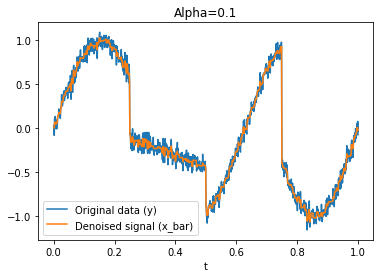
\includegraphics[width=1\columnwidth]{Images/3a01.png}
		\label{3a01}
	\end{subfigure}
	\begin{subfigure}[b]{0.45\textwidth}
		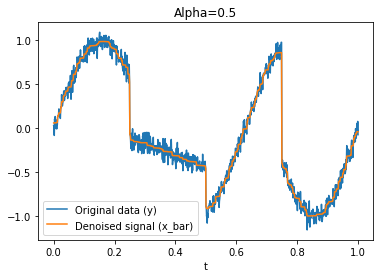
\includegraphics[width=1\columnwidth]{Images/3a05.png}
		\label{3a05}
	\end{subfigure}
	\begin{subfigure}[b]{0.45\textwidth}
		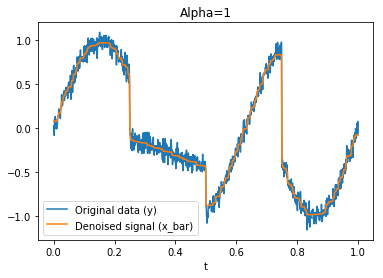
\includegraphics[width=1\columnwidth]{Images/3a1.png}
		\label{3a1}
	\end{subfigure}
	\begin{subfigure}[b]{0.45\textwidth}
		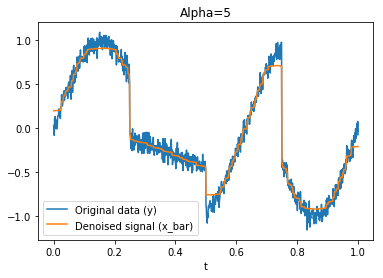
\includegraphics[width=1\columnwidth]{Images/3a5.png}
		\label{3a5}
	\end{subfigure}
	\caption{Ergebnisse des angepassten Frank-Wolfe-Verfahrens aus Aufgabenteil c) für $\bar{x}$ aus $RL_1$ mit $\alpha \in \{\frac{1}{10}, \frac{1}{2}, 1, 5\}$.}
	\vspace{-20pt}
\end{figure}
\par
(e) Der Ansatz aus Teilaufgabe d) ist im vorliegenden Fall besser als der Ansatz aus Aufgabe S2.2 geeignet um das zufälliger Rauschen aus den Messwerten zu entfernen. Dies liegt daran, dass der Datensatz Sprünge aufweist die kaum über das natürliche rauschen zu erklären sind. Der Ansatz aus Teilaufgabe d) ist dabei besser geeignet als der Ansatz aus S2.2, da er die Sprungstellen in den Daten verbleiben lässt, wohingegen der Ansatz aus S2.2 zu einer quasi-glatten Funktion führt. Die Unterschiedlichen Ergebnisse sind ein Resultat der verschiedenen Normen der Regularisierungs-Terme. Die quadrierte Euklidische Norm aus S2.2 bestraft große Sprünge besonders stark (quadratisch) und versucht daher sie tendenziell \glqq zu vermeiden\grqq, wohin gegen die 1-Norm aus Teilaufgabe d) nur die absolute Sprunghöhe bestraft und die Sprünge daher tendenziell zunächst \glqq beibehällt\grqq ~(merke das sich bei beiden Normen mit steigendem $\alpha$ die Ergebnisse einer horizontalen Geraden um den Mittelwert annähern). Dies entspricht auch den Ergebnisse aus Aufgabe S1.2d, bei der ebenfalls die Unterschiedlichen Auswirkungen von Ausreißern (hier analog zu den Sprungstellen) auf die 1-Norm und die quadrierte euklidische Norm gezeigt worden sind. Auch dort hat die quadrierte euklidische Norm deutlich stärker auf Aussreißer reagiert und die 1-Norm sich robuster verhalten.
\par
\end{document}